Das  Herzst\"uck des  Versuches  bildet eine  zylindrische Kupferspule  (Draht
aufgewickelt  auf  einen  Acrylglas-Zylinder),  in  deren  Mitte  eine  kleine
\"Offnung   eingelassen  ist,   durch   die  eine   Messsonde  senkrecht   zur
Zylinderachse eingef\"uhrt werden kann.

In  diese Zylinderspule  werden die  Versuchsproben axial  eingef\"uhrt (Hohl-
oder Vollzylinder),  wobei diese  ebenfalls Aussparungen in  radialer Richtung
f\"ur das Einf\"uhren  der Messsonde aufweisen. Der Vollzylinder  ist dabei in
zwei H\"alften (geschnitten im Querschnitt) ausgew\"uhrt.

Der  Messbereich  ist axial  zentriert,  um  Randeffekte beim  Magnetfeld  der
Zylinderspule vernachl\"assigen zu k\"onnen.

Der  Messsensor  ist  an  einer Schublehre  (auch  bekannt  als  Messschieber)
angebracht, womit seine radiale Position gemessen werden kann.

Die Einheit der Messwerte, welche das Oszilloskop an den Benutzer ausgibt, ist
Volt, daher wird diese auch auf s\"amtlichen Tabellen und Plots benutzt. Da es
beim Versuch  um das Fitten von  Kurven in ihrer \emph{Form}  an Messwerte und
nicht  um  die absoluten  Werte  des  B-Feldes  geht,  ist dies  nicht  weiter
tragisch.


% **************************************************************************** %
\subsection{Versuchsanordnung}
\label{sec:durchf:subsec:anordn}
% **************************************************************************** %

\begin{figure}[!htb]
    \resizebox{\textwidth}{!}{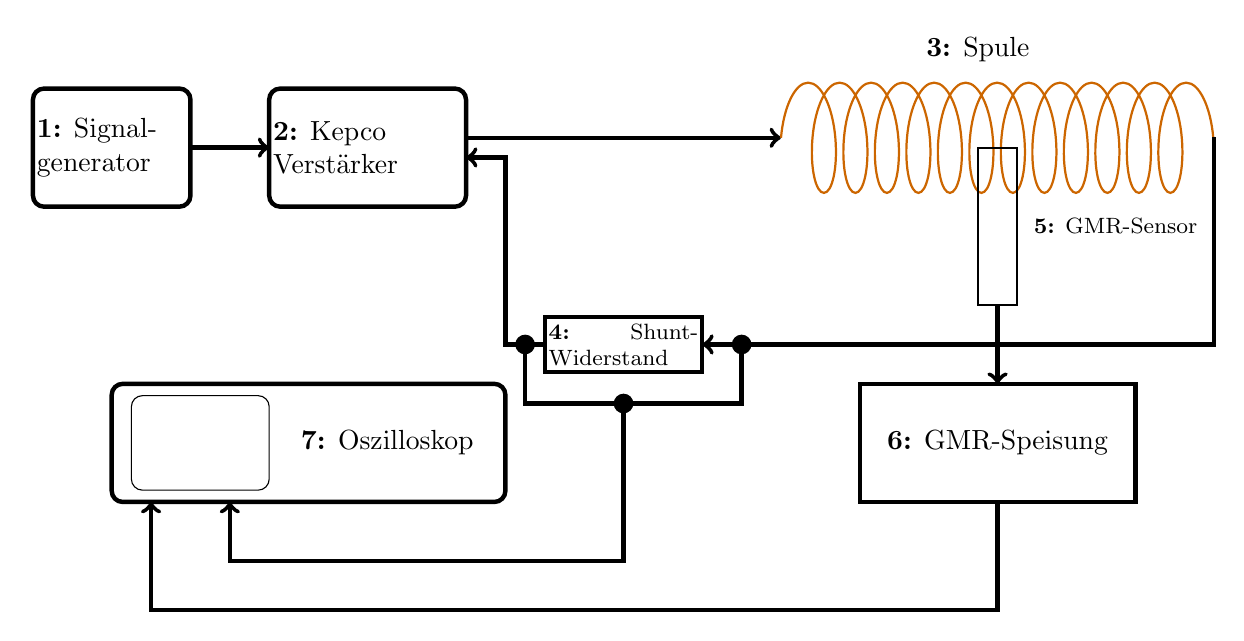
\begin{tikzpicture}

    % signal generator
    \draw[black,ultra thick,rounded corners] (0,0) rectangle (2,1.5);
    \node at (1,.75) {\parbox{1.9cm}{\textbf{1:} Signal-\\generator}};

    % line from signal generator to amplifier
    \draw[->,ultra thick] (2,.75) -- (3,.75);

    % amplifier
    \draw[black,ultra thick,rounded corners] (3,0) rectangle (5.5,1.5);
    \node at (4,.75) {\parbox{1.9cm}{\textbf{2:} Kepco \\ Verst\"arker}};

    % line from amplifier to coil
    \draw[->,ultra thick] (5.5,.75+.125) -- (9.5,.75+.125);

    % coil
    \draw[thick,color=orange!80!black,decoration={aspect=0.35, segment length=4mm, amplitude=7mm,coil},decorate] (9.5,.75+.125) -- (15,.75+.125);
    \node at (12,2) {\textbf{3:} Spule};

    % line from right side of coil to shunt resistor
    \draw[->,ultra thick] (15,.76+.125) -- (15,-1.75) -- (8.5,-1.75);

    % shunt resistor
    \draw[black,ultra thick] (6.5,-1.75+.7/2) rectangle (8.5,-1.75-.7/2);
    \node at (7.5,-1.75) {\footnotesize\parbox{1.9cm}{\textbf{4:} Shunt-Widerstand}};

    % line from shunt resistor to amplifier
    \draw[->,ultra thick] (6.5,-1.75) -- (6,-1.75) -- (6,.75-.125) -- (5.5,.75-.125);

    % GMR sensor
    \draw[black,thick] (12,0.75) rectangle (12.5,-1.25);
    \node at (13.75,-0.25) {\footnotesize{\textbf{5:} GMR-Sensor}};

    % line from GMR sensor to GMR box
    \draw[->,ultra thick] (12.25,.-1.25) -- (12.25,-2.25);

    % GMR box
    \draw[black,ultra thick] (14,-2.25) rectangle (10.5,-3.75);
    \node at (12.25,-3) {\textbf{6:} GMR-Speisung};

    % line from GMR box to oscilloscope
    \draw[->,ultra thick] (12.25,-3.75) -- (12.25,-5-.125) -- (1.5,-5-.125) -- (1.5,-3.75);

    % oscilloscpe
    \draw[black,ultra thick,rounded corners] (6,-2.25) rectangle (1,-3.75);
    \draw[black,rounded corners] (3,-2.4) rectangle (1.25,-3.6);
    \node at (4.5,-3) {\textbf{7:} Oszilloskop};

    % Measurement of shunt voltage
    \draw[-,ultra thick] (6.25,-1.75) -- (6.25,-2.5) -- (7.5-.125,-2.5);
    \draw[-,ultra thick] (9,-1.75) -- (9,-2.5) -- (7.5+.125,-2.5);
    \fill (7.5,-2.5) circle [radius=0.125];
    \draw[->,ultra thick] (7.5,-2.5) -- (7.5,-4.5)  -- (2.5,-4.5) -- (2.5,-3.75);
    \draw[-,ultra thick] (6.25 - 0.025,-2.5) -- (8.75 + 0.025,-2.5);
    \fill (6.25,-1.75) circle [radius=0.125];
    \fill (9,-1.75) circle [radius=0.125];
\end{tikzpicture}
}
    \caption{Versuchsanordnung, schematisch}
    \label{fig:versuch:schematic}
\end{figure}

Im  Vergleich   zur  Versuchsanleitung   wurde  die   Versuchsapparatur  etwas
aktualisiert (insbesondere wurde das  Oszilloskop durch ein moderneres Ger\"at
ersetzt), daher  ist das  dortige Schema des  Versuchsaufbaus nicht  mehr ganz
aktuell. Abbildung \ref{fig:versuch:schematic} enth\"ahlt  deshalb ein Schema,
das dem Aufbau am Tag des Versuchs entspricht (Abbildungen \ref{fig:versuch:1}
und \ref{fig:versuch:2}).

Die Nummerierung der Ger\"ate  in den Abbildungen \ref{fig:versuch:schematic},
\ref{fig:versuch:1} und  \ref{fig:versuch:2} und  in der  folgenden Auflistung
ist konsistent.

\begin{figure}[!htb]
    \resizebox{\textwidth}{!}{%\begin{tikzpicture}[scale=2.2,transform shape]
\begin{tikzpicture}
    \node[anchor=south west,inner sep=0] at (0,0)
        {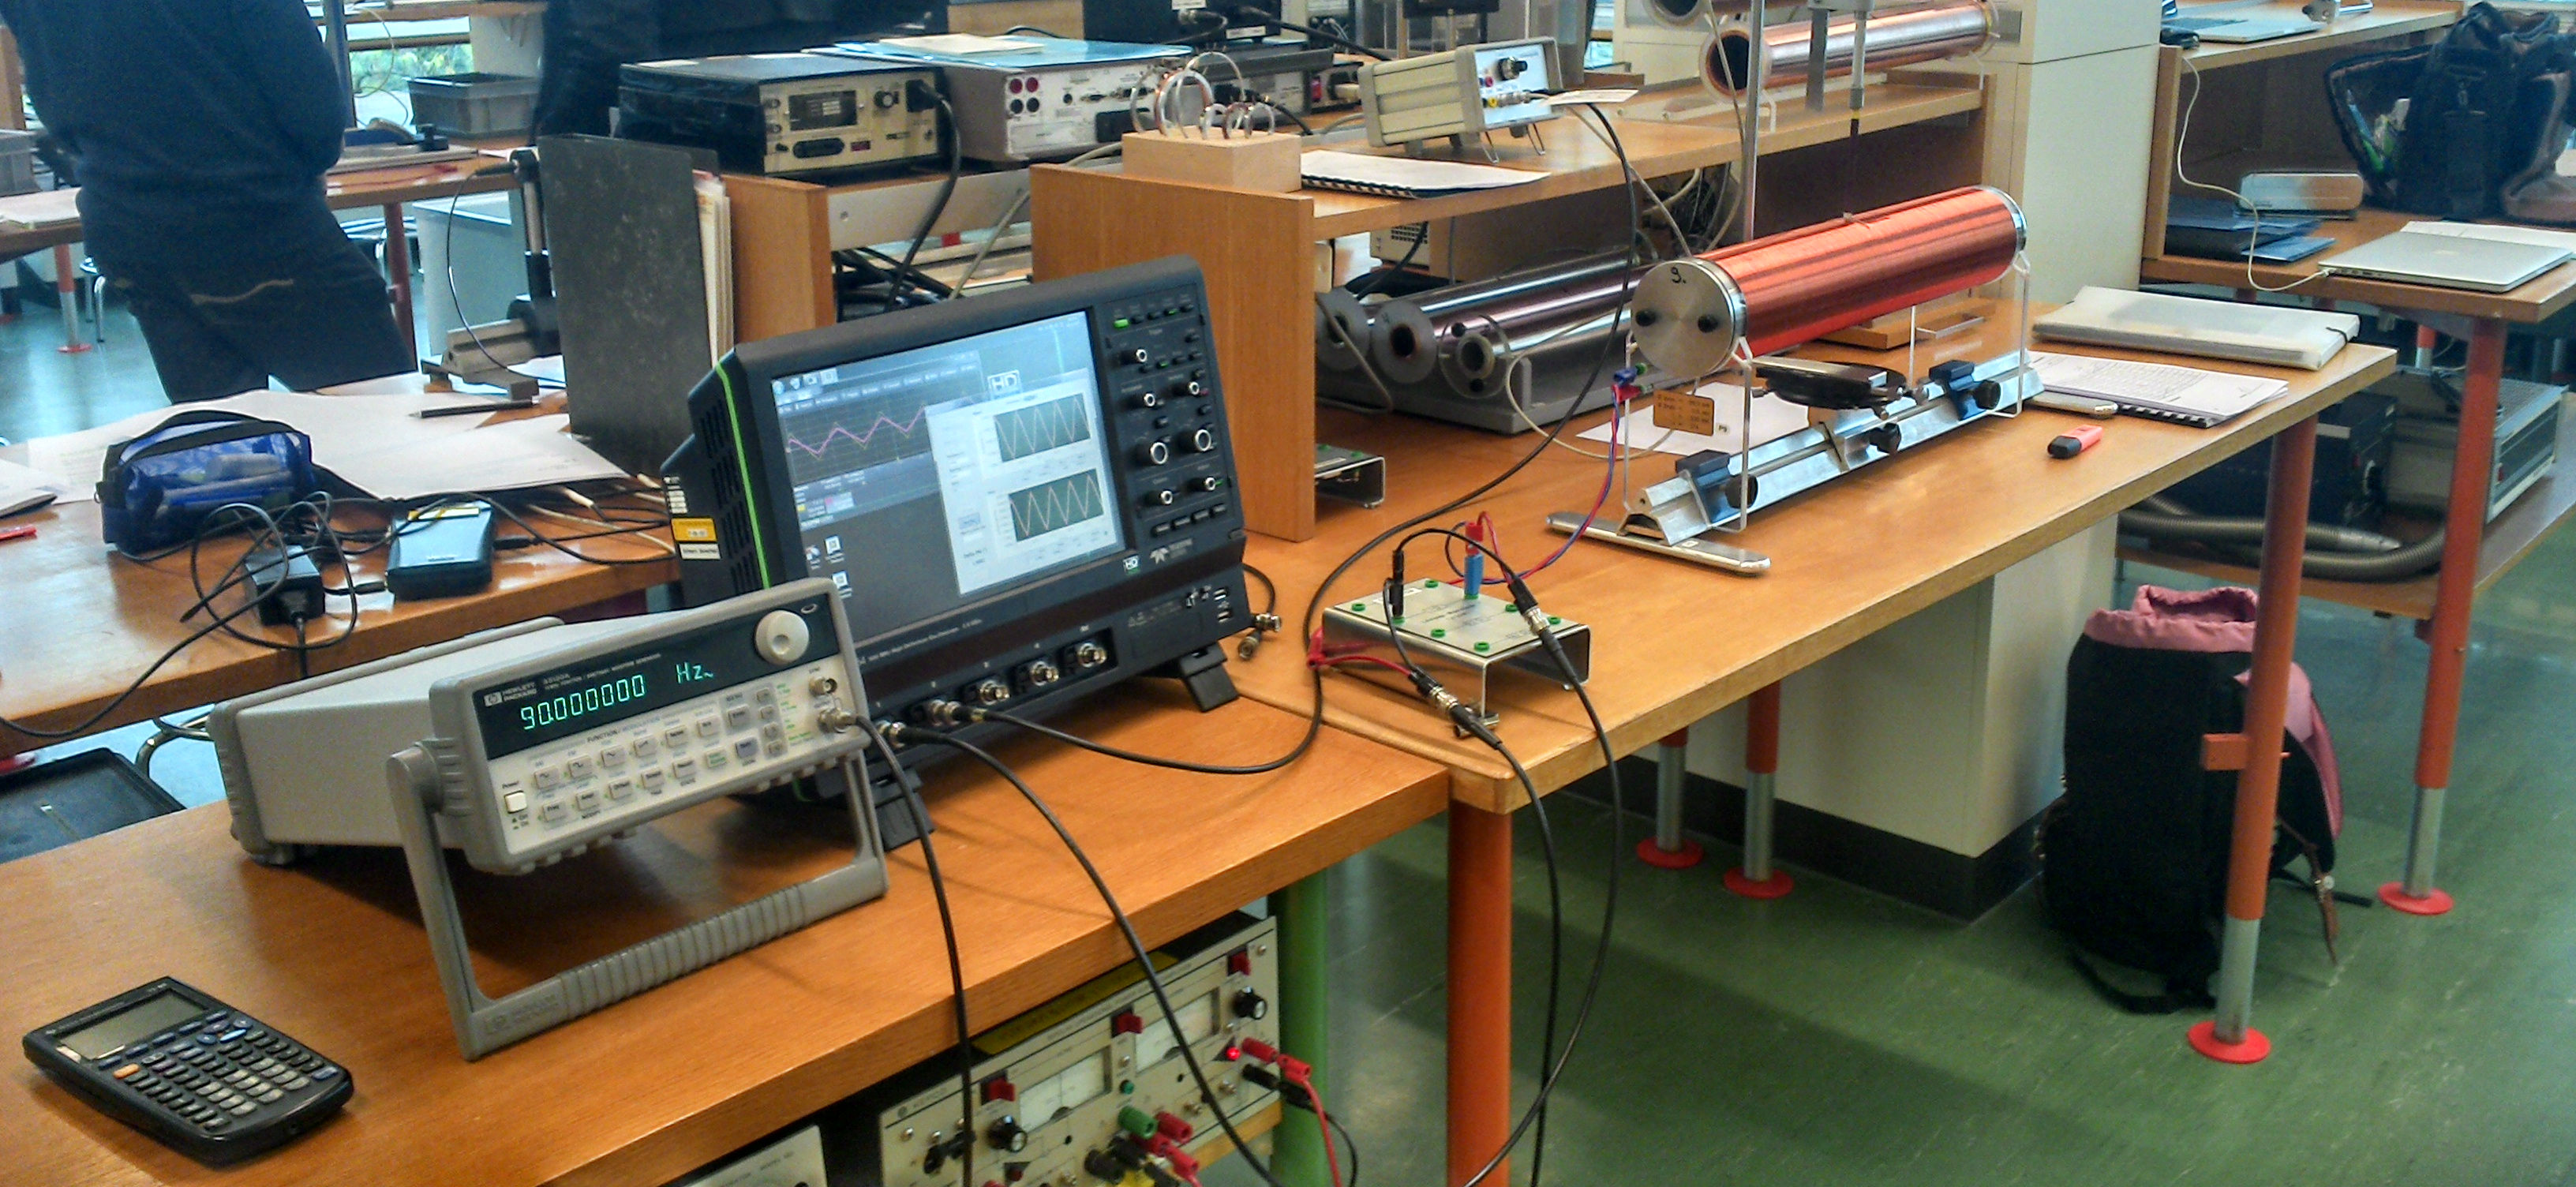
\includegraphics[width=\textwidth]{images/versuchsanordnung-1.jpeg}};

    %\draw[help lines] (0,0) grid (\textwidth,7);

    \fill[black,opacity = 0.6,rounded corners] (1,1) rectangle (1.6,1.8);
    \draw[white,ultra thick,rounded corners] (1,1) rectangle (5,3.45);
    \node at (1.3,1.4) {\huge{\textcolor{white}{1}}};

    \fill[black,opacity = 0.6,rounded corners] (6.4,2) rectangle (7,2.8);
    \draw[green,ultra thick,rounded corners] (4,2) rectangle (7,5);
    \node at (6.7,2.4) {\huge{\textcolor{green}{7}}};

    \fill[black,opacity = 0.6,rounded corners] (8.8,2.5) rectangle (9.4,3.3);
    \draw[yellow,ultra thick,rounded corners] (7.1,2.5) rectangle (9.4,3.6);
    \node at (9.1,2.9) {\huge{\textcolor{yellow}{4}}};

    \fill[white,opacity = 0.6,rounded corners] (11,4) rectangle (11.6,4.8);
    \draw[black,ultra thick,rounded corners] (8.5,4) rectangle (11.6,5.7);
    \node at (11.28,4.4) {\huge{\textcolor{black}{3}}};
\end{tikzpicture}
}
    \caption{Versuchsanordnung}
    \label{fig:versuch:1}
\end{figure}
\begin{figure}[!htb]
    \resizebox{\textwidth}{!}{%\begin{tikzpicture}[scale=2.2,transform shape]
\begin{tikzpicture}
    \node[anchor=south west,inner sep=0] at (0,0)
        {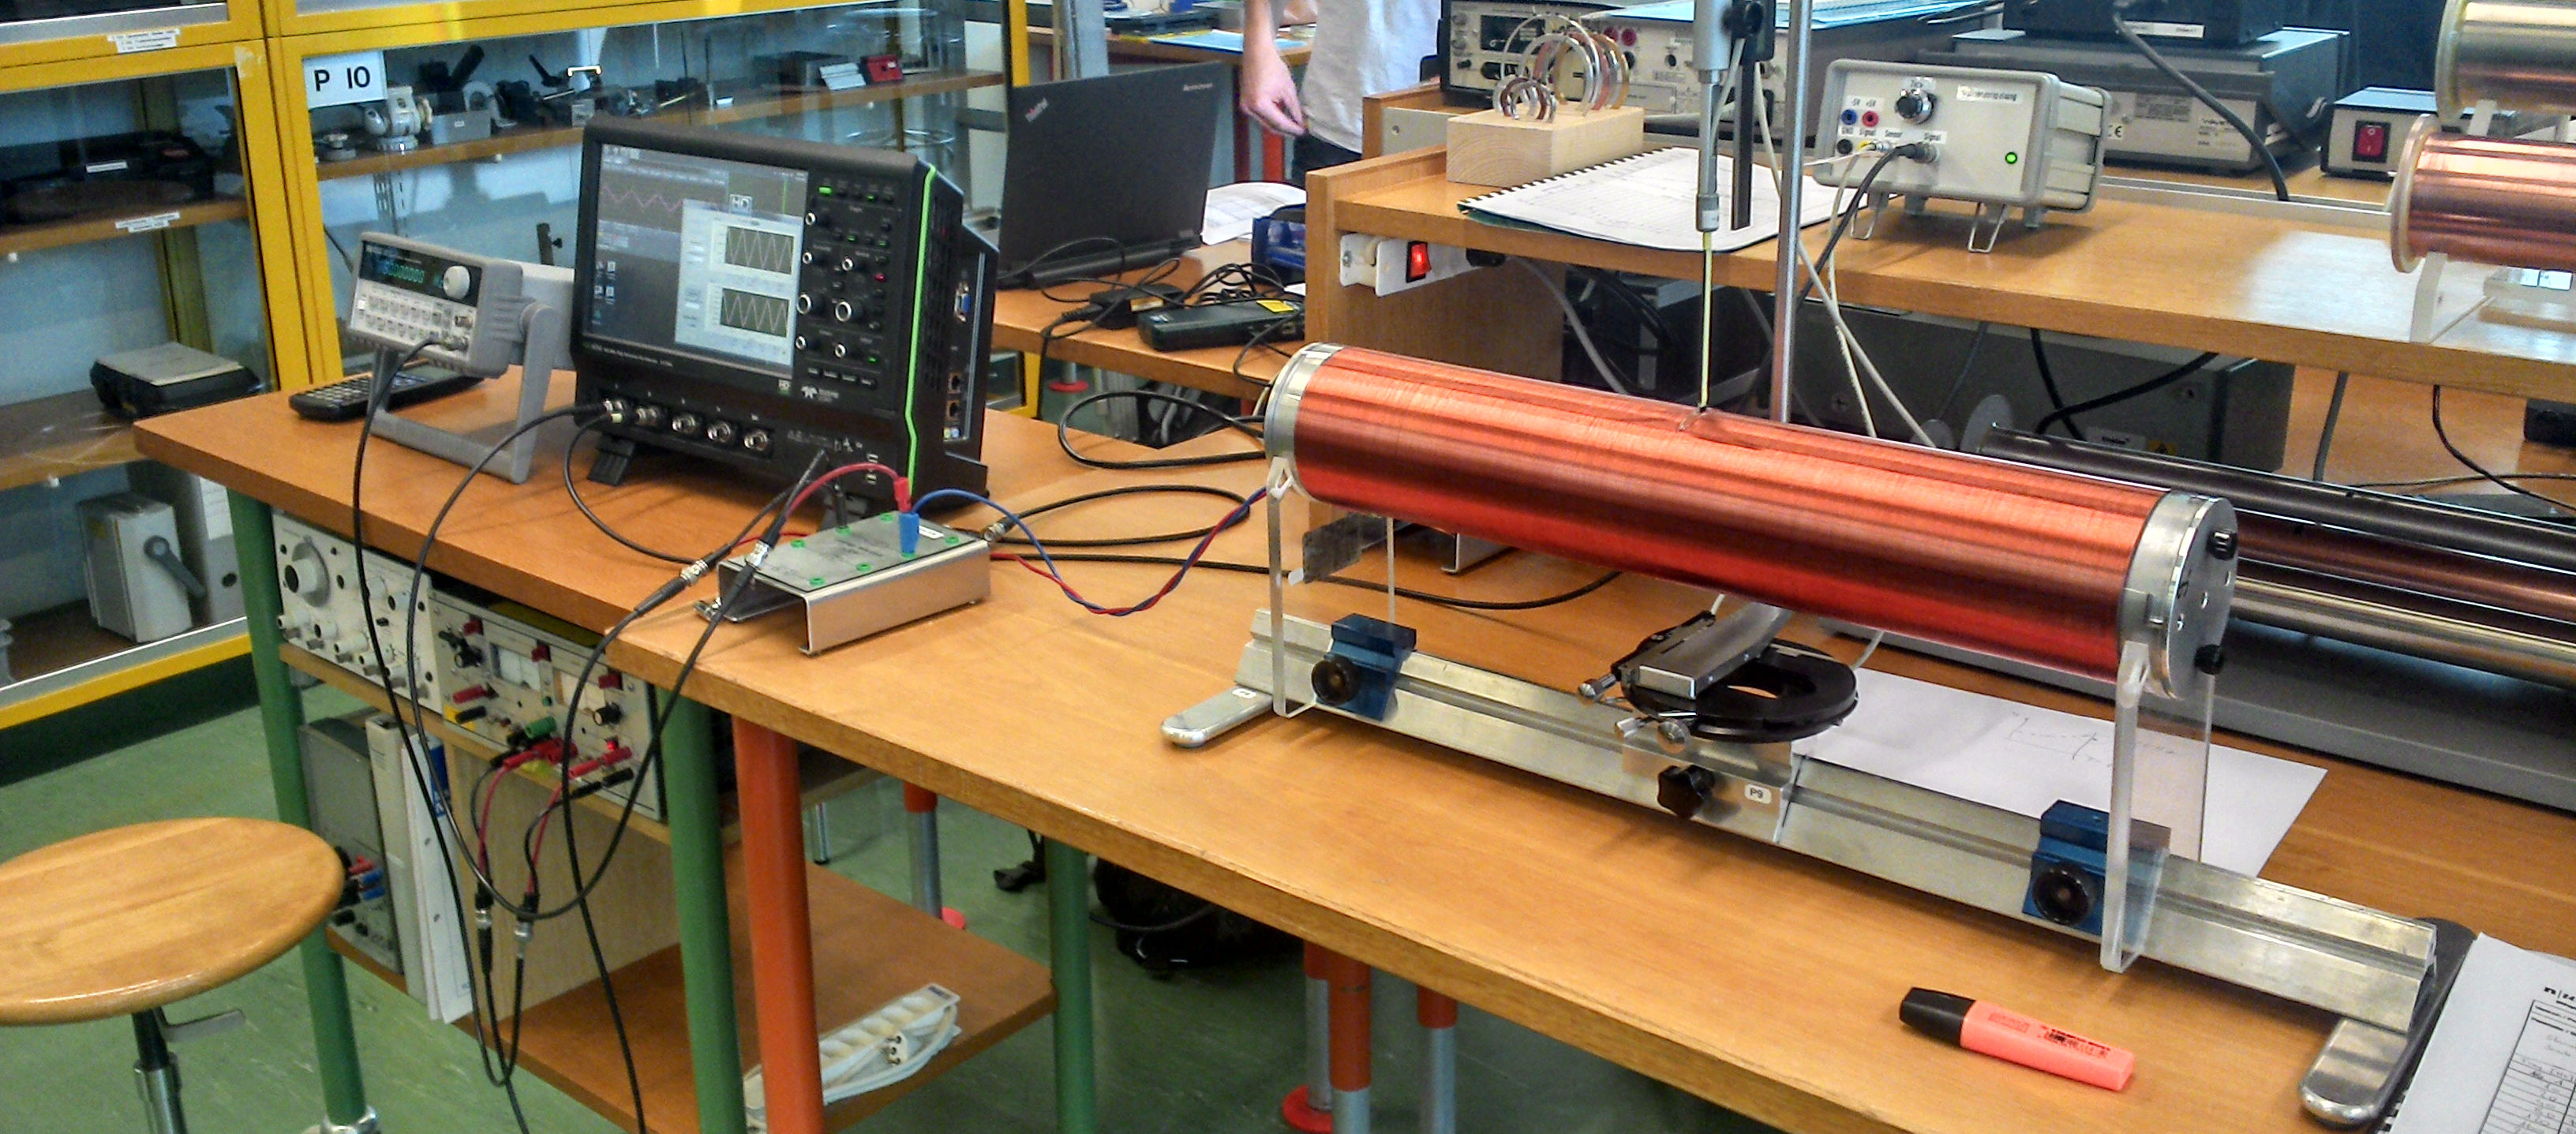
\includegraphics[width=\textwidth]{images/versuchsanordnung-2.jpeg}};

    %\draw[help lines] (0,0) grid (\textwidth,7);

    \fill[black,opacity = 0.6,rounded corners] (1.6,1.7) rectangle (2.2,2.5);
    \draw[white,ultra thick,rounded corners] (1.6,1.7) rectangle (4,3);
    \node at (1.9,2.15) {\huge{\textcolor{white}{2}}};

    \fill[black,opacity = 0.6,rounded corners] (8,4.5) rectangle (9,5.3);
    \draw[green,ultra thick,rounded corners] (8,4.5) rectangle (11.6,5.9);
    \node at (8.5,4.875) {\huge{\textcolor{green}{5,6}}};
\end{tikzpicture}
}
    \caption{Versuchsanordnung}
    \label{fig:versuch:2}
\end{figure}

Die verwendeten Ger\"ate waren:
\begin{enumerate}
    \item
        Signalgenerator: Hewlett-Packard 33120A
    \item
        Verst\"arker: Kepco Bipolar Operational Power Supply/Amplifier P-E-102
    \item
        Zylinderspule aus Kupferdraht:
        \begin{itemize}
            \item
               $\SI{98}{\milli\meter}$ Innendurchmesser
           \item
               $\SI{0.8}{\milli\meter}$ Drahtdurchmesser
           \item
               $\SI{500}{\milli\meter}$ L\"ange
           \item
               $\num{574}$ Windungen
        \end{itemize}
    \item
        Shunt-Widerstand: $\SI{1}{\ohm}$, $\SI{50}{\watt}$
    \item
        GMR-Sonde Honeywell SS94A1F
    \item
        GMR-Speisebox zugeh\"orig zu Sonde Honeywell SS94A1F
    \item
        Oszilloskop: Teledyne Lecroy HD06054
\end{enumerate}


% **************************************************************************** %
\subsection{Messvorgang/Messmethoden}
\label{sec:durchf:subsec:messmethoden}
% **************************************************************************** %


Bei  der Messung  wurde jeweils  eine Messprobe  ins Innere  der Zylinderspule
eingef\"uhrt   wie  in   den  Abbildungen   \ref{fig:looser:vollzylinder}  und
\ref{fig:looser:hohlzylinder3d}  auf  Seite  \pageref{fig:looser:vollzylinder}
respektive \pageref{fig:looser:hohlzylinder3d} dargestellt.

Anschliessend   wurden  folgende   Messungen   zur   Erfassung  des   B-Feldes
durchgef\"uhrt:

\begin{itemize}
    \item
        Vollzylinder Aluminium:
        \begin{itemize}
            \item
                Frequenzgang,   GMR-Sonde    axial   und    radial   zentriert
                (Abbildung~\ref{fig:sensor:fixed})
            \item
                \"uber   den  ganzen   Radius   variierende  Position,   axial
                zentriert, bei  fixierter tiefer  Frequenz ($\SI{30}{\hertz}$)
                (Abbildung~\ref{fig:sensor:radial:full}) und
            \item
                \"uber     die      \"aussere     H\"alfte      des     Radius
                variierende      Position,      axial      zentriert,      bei
                fixierter       hoher      Frequenz       ($\SI{450}{\hertz}$)
                (Abbildung~\ref{fig:sensor:radial:partial}).
        \end{itemize}
    \item
        Hohlzylinder Kupfer:
        \begin{itemize}
            \item
                Frequenzgang,   GMR-Sonde    axial   und    radial   zentriert
                (Abbildung~\ref{fig:sensor:fixed})
        \end{itemize}
    \item
        Hohlzylinder rostfreier Stahl:
        \begin{itemize}
            \item
                Frequenzgang,   GMR-Sonde    axial   und    radial   zentriert
                (Abbildung~\ref{fig:sensor:fixed})
        \end{itemize}
\end{itemize}

\begin{minipage}[t]{.33\textwidth}
    \vspace{0mm}
    \resizebox{\textwidth}{!}{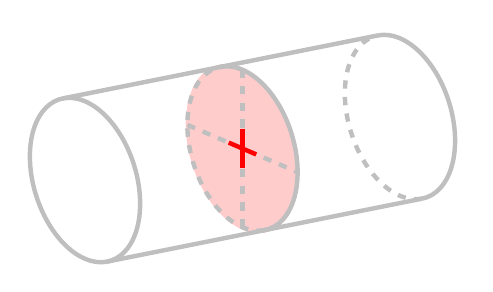
\begin{tikzpicture}
    \begin{scope}[x={(.7cm,-.3cm)},z={(-.5cm,-.1cm)}]
        \path (1,0,0);
        \pgfgetlastxy{\cylxx}{\cylxy}
        \path (0,1,0);
        \pgfgetlastxy{\cylyx}{\cylyy}
        \path (0,0,1);
        \pgfgetlastxy{\cylzx}{\cylzy}
        \pgfmathsetmacro{\cylt}{(\cylzy * \cylyx - \cylzx * \cylyy)/ (\cylzy * \cylxx - \cylzx * \cylxy)}
        \pgfmathsetmacro{\ang}{atan(\cylt)}
        \pgfmathsetmacro{\ct}{1/sqrt(1 + (\cylt)^2)}
        \pgfmathsetmacro{\st}{\cylt * \ct}
        \fill[red!20] (0,0,-4) circle[radius=1.03];
        \begin{scope}[every path/.style={ultra thick,black!25}]

            % front ellipse
            \draw (0,0,0) circle[radius=1];

            % middle ellipse
            \draw (\ct,\st,-4) arc[start angle=\ang,delta angle=180,radius=1];
            \draw[dashed] (\ct,\st,-4) arc[start angle=\ang,delta angle=-180,radius=1];

            % measurement marker in middle of central axis
            \draw[dashed] (-1,0,-4) -- (1,0,-4);
            \draw[dashed] (0,-1,-4) -- (0,1,-4);
            \draw[-][red] (-.25,0,-4) -- (.25,0,-4);
            \draw[-][red] (0,-.25,-4) -- (0,.25,-4);

            % Cylinder Edges
            \draw (\ct,\st,0) -- ++(0,0,-8);
            \draw (-\ct,-\st,0) -- ++(0,0,-8);

            % back ellipse
            \draw (\ct,\st,-8) arc[start angle=\ang,delta angle=180,radius=1];
            \draw[dashed] (\ct,\st,-8) arc[start angle=\ang,delta angle=-180,radius=1];
        \end{scope}
    \end{scope}
\end{tikzpicture}
%source: http://tex.stackexchange.com/questions/31548/drawing-simple-3d-cylinders-in-tikz
}
    \captionof{figure}{Sonde ist axial und radial zentriert fixiert.}
    \label{fig:sensor:fixed}
\end{minipage}%
\begin{minipage}[t]{.33\textwidth}
    \vspace{0mm}
    \resizebox{\textwidth}{!}{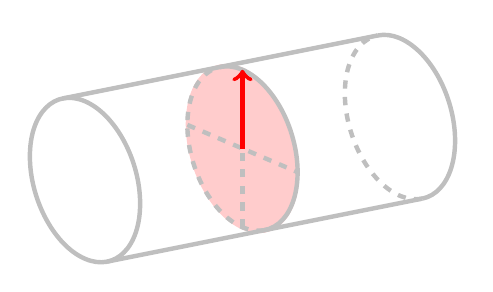
\begin{tikzpicture}
    \begin{scope}[x={(.7cm,-.3cm)},z={(-.5cm,-.1cm)}]
        \path (1,0,0);
        \pgfgetlastxy{\cylxx}{\cylxy}
        \path (0,1,0);
        \pgfgetlastxy{\cylyx}{\cylyy}
        \path (0,0,1);
        \pgfgetlastxy{\cylzx}{\cylzy}
        \pgfmathsetmacro{\cylt}{(\cylzy * \cylyx - \cylzx * \cylyy)/ (\cylzy * \cylxx - \cylzx * \cylxy)}
        \pgfmathsetmacro{\ang}{atan(\cylt)}
        \pgfmathsetmacro{\ct}{1/sqrt(1 + (\cylt)^2)}
        \pgfmathsetmacro{\st}{\cylt * \ct}
        \fill[red!20] (0,0,-4) circle[radius=1.03];
        \begin{scope}[every path/.style={ultra thick,black!25}]

            % front ellipse
            \draw (0,0,0) circle[radius=1];

            % middle ellipse
            \draw (\ct,\st,-4) arc[start angle=\ang,delta angle=180,radius=1];
            \draw[dashed] (\ct,\st,-4) arc[start angle=\ang,delta angle=-180,radius=1];

            % measurement marker in middle of central axis
            \draw[dashed] (-1,0,-4) -- (1,0,-4);
            \draw[dashed] (0,-1,-4) -- (0,1,-4);

            % measurement line
            \draw[->][red] (0,0,-4) -- (0,1,-4);

            % Cylinder Edges
            \draw (\ct,\st,0) -- ++(0,0,-8);
            \draw (-\ct,-\st,0) -- ++(0,0,-8);

            % back ellipse
            \draw (\ct,\st,-8) arc[start angle=\ang,delta angle=180,radius=1];
            \draw[dashed] (\ct,\st,-8) arc[start angle=\ang,delta angle=-180,radius=1];
        \end{scope}
    \end{scope}
\end{tikzpicture}
%source: http://tex.stackexchange.com/questions/31548/drawing-simple-3d-cylinders-in-tikz
}
    \captionof{figure}{Sonde l\"auft den gesamten Radius ab, axial zentriert.}
    \label{fig:sensor:radial:full}
\end{minipage}%
\begin{minipage}[t]{.33\textwidth}
    \vspace{0mm}
    \resizebox{\textwidth}{!}{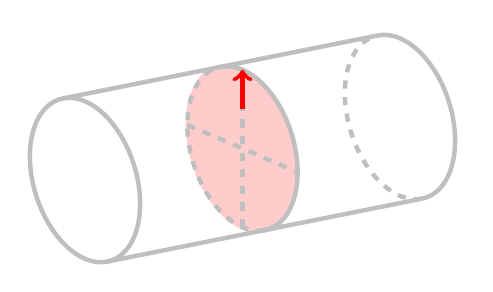
\begin{tikzpicture}
    \begin{scope}[x={(.7cm,-.3cm)},z={(-.5cm,-.1cm)}]
        \path (1,0,0);
        \pgfgetlastxy{\cylxx}{\cylxy}
        \path (0,1,0);
        \pgfgetlastxy{\cylyx}{\cylyy}
        \path (0,0,1);
        \pgfgetlastxy{\cylzx}{\cylzy}
        \pgfmathsetmacro{\cylt}{(\cylzy * \cylyx - \cylzx * \cylyy)/ (\cylzy * \cylxx - \cylzx * \cylxy)}
        \pgfmathsetmacro{\ang}{atan(\cylt)}
        \pgfmathsetmacro{\ct}{1/sqrt(1 + (\cylt)^2)}
        \pgfmathsetmacro{\st}{\cylt * \ct}
        \fill[red!20] (0,0,-4) circle[radius=1.03];
        \begin{scope}[every path/.style={ultra thick,black!25}]

            % front ellipse
            \draw (0,0,0) circle[radius=1];

            % middle ellipse
            \draw (\ct,\st,-4) arc[start angle=\ang,delta angle=180,radius=1];
            \draw[dashed] (\ct,\st,-4) arc[start angle=\ang,delta angle=-180,radius=1];

            % measurement marker in middle of central axis
            \draw[dashed] (-1,0,-4) -- (1,0,-4);
            \draw[dashed] (0,-1,-4) -- (0,1,-4);

            % measurement line
            \draw[->][red] (0,0.5,-4) -- (0,1,-4);

            % Cylinder Edges
            \draw (\ct,\st,0) -- ++(0,0,-8);
            \draw (-\ct,-\st,0) -- ++(0,0,-8);

            % back ellipse
            \draw (\ct,\st,-8) arc[start angle=\ang,delta angle=180,radius=1];
            \draw[dashed] (\ct,\st,-8) arc[start angle=\ang,delta angle=-180,radius=1];
        \end{scope}
    \end{scope}
\end{tikzpicture}
%source: http://tex.stackexchange.com/questions/31548/drawing-simple-3d-cylinders-in-tikz
}
    \captionof{figure}{Sonde l\"auft den halben Radius ab, axial zentriert.}
    \label{fig:sensor:radial:partial}
\end{minipage}


% **************************************************************************** %
\clearpage
\subsection{Proben}
\label{sec:durchf:subsec:proben}
% **************************************************************************** %


Es wurden drei Versuchsobjekte benutzt:
\begin{itemize}
    \item
        Hohlzylinder aus Kupfer:
        \begin{itemize}
            \item
                $\SI{70}{\milli\meter}$ Aussendurchmesser
            \item
                $\SI{60}{\milli\meter}$ Innendurchmesser
            \item
                $\SI{500}{\milli\meter}$ L\"ange
        \end{itemize}
    \item
        Hohlzylinder aus rostfreiem Stahl:
        \begin{itemize}
            \item
                $\SI{70}{\milli\meter}$ Aussendurchmesser
            \item
                $\SI{60}{\milli\meter}$ Innendurchmesser
            \item
                $\SI{500}{\milli\meter}$ L\"ange
        \end{itemize}
    \item
        Vollzylinder aus Aluminium:
        \begin{itemize}
            \item
                $\SI{90}{\milli\meter}$ Durchmesser
            \item
                $\SI{500}{\milli\meter}$ L\"ange (verteilt auf zwei H\"alften)
        \end{itemize}
\end{itemize}


Die  Leitwerte der  Proben waren  nicht  bekannt und  sollten via  Fit an  die
Messpunkte  bestimmt werden. Dabei  ist zu  beachten, dass  die Literaturwerte
und die  experimentell bestimmten  Werte betr\"achtlich  voneinander abweichen
k\"onnen   (je  nach   Herstellungsprozess   k\"onnen  Metalle,   insbesondere
Aluminium, stark  variierende elektrische  Leitf\"ahigkeiten aufweisen).


% **************************************************************************** %
\subsection{Messungen}
\label{sec:durchf:subsec:ablauf}
% **************************************************************************** %


Die Messwerte wurden auf dem  Oszilloskop mit einer vom Dozenten geschriebenen
Spezialsoftware ausgelesen. Diese wertet dabei die rohen Messpunkte (Spannung,
welche von der GMR-Sonde via  Speiseger\"at an das Oszilloskop geliefert wird)
aus und errechnet einen passenden Fit an diese Spannungswerte.

Die Amplitude  dieses Fits  sowie die Phasenverschiebung  zwischen dem  Fit an
die  GMR-Messwerte  und dem  Fit  an  die  zum \"ausseren  B-Feld geh\"orenden
Messwerte (repr\"asentiert  durch die Shunt-Spannung) werden  anschliessend an
den Benutzer  ausgegeben. Es sind diese  Werte, welche in  den Messprotokollen
erfasst sind.

Die Shunt-Spannung wurde konstant  bei $\SI{200}{\milli\volt}$ gehalten (somit
der  Spulen-Strom  bei  $\SI{200}{\milli\ampere}$. Bei  der  ersten  Messreihe
wurde sie  zur Kontrolle erfasst,  anschliessend nicht mehr.   Die ermittelten
Messwerte sind in Tabelle \ref{tab:meas:copper:shunt} zu finden.

\clearpage
\begin{center}
    \captionof{table}{%
        Frequenz und  Shunt-Spannung beim  Frequenzgang von  Zylinderspule mit
        Kupferrohr
    }
    \label{tab:meas:copper:shunt}
    \sisetup{math-rm=\mathtt}
    \begin{tabular}{%
        S[table-number-alignment=right]
        S[table-number-alignment=right]
        S[table-number-alignment=right]
        S[table-number-alignment=right]
        }
        \toprule
        {Frequenz ($\si{\hertz}$)}             &
        {$V_{R_{Shunt}}$ ($\si{\milli\volt}$)} &
        {Frequenz ($\si{\hertz}$)}             &
        {$V_{R_{Shunt}}$ ($\si{\milli\volt}$)} \\
        \midrule
           1 & 195.3 & 200 & 200.0 \\
          10 & 200.0 & 400 & 200.0 \\
          20 & 200.0 & 600 & 199.7 \\
          40 & 200.3 & 800 & 200.5 \\
          80 & 200.0 &1000 & 200.2 \\
         120 & 200.1 &1200 & 200.0 \\
         160 & 200.1 &1500 & 199.9 \\
        \bottomrule
    \end{tabular}
\end{center}
Bei gewissen Versuchen  schwankten die ausgegebenen Werte  merklich (die Phase
war  davon st\"arker  betroffen als  die  Amplitude), was  ein gutes  Auslesen
zeitweise  erschwerte. Bei  den  betroffenen  Messungen ist  dies  im  Kapitel
\emph{Auswertung} jeweils angemerkt.

Im Allgemeinen  war das Durchf\"uhren  des Versuches dank der  Software jedoch
eine  komfortable Angelegenheit,  und  wie  man sehen  wird,  decken sich  die
ermittelten Messwerte im Grossen und  Ganzen zufriedenstellend mit der Theorie
und sind anscheinend von guter Qualit\"at.

Die   Messprotokolle    sind   in   Anhang   \ref{app:protocols}    ab   Seite
\pageref{app:protocols} zu finden.
